%Update 9/7/2022
\documentclass{article}     %type of document
\usepackage[utf8]{inputenc} %for text encoding
\usepackage{../lambdatex} 
\everymath{\displaystyle}

\title{Limiti}
\author{Davide Borra - 5LA}
\date{A.S. 2021-2022}

\begin{document}

\begin{titlepage}
    \maketitle
    \tableofcontents
    \vspace{\fill}
    \hspace{\fill} v. 1.2   %incrementare primo numero per contenuti e secondo numero per patch
\end{titlepage}

\lhead{Teoremi di Analisi}
\chead{}
\rhead{Davide Borra - 5LA}
\section{Intervalli in $\R$}
\begin{definition}
    Un insieme $A \subset \R$ si dice \textbf{intervallo} se corrisponde ad una semiretta (\textbf{illimitato}) o ad un segmento (\textbf{limitato}) della retta reale
\end{definition}
Inoltre:
\begin{itemize}
    \item si dice \textbf{chiuso} se gli estremi sono inclusi nell'intervallo;
    \item si dice \textbf{aperto} se gli estremi sono esclusi nell'intervallo.
\end{itemize}
Gli intervallo limitati corrispondono a segmenti di retta reale di estremi $a$ e $b$ ($b>a$), lunghezza $b-a$ (detta \textbf{ampiezza} dell'intervallo), \textbf{centro} $\frac{b+a}{2}$ e \textbf{raggio} $\frac{b-a}{2}$.
\subsection{Intorni}
\begin{definition}
    Dato numero reale $x_0$, un intorno completo di $x_0$ è un qualunque intervallo aperto contenente $x_0$ \[I(x_0)=]x_0-\delta_1;x_0+\delta_2[ ~~~~~~ (con \delta_1, \delta_2 \in \R_0^+\]
\end{definition}
\begin{enumerate}
    \item \textbf{intorno destro}: $I^+(x_0)=]x_0;x_0+\delta[$
    \item \textbf{intorno sinistro}: $I^-(x_0)=]x_0-\delta;x_0[$
\end{enumerate}
\subsubsection{Intorni circolari}
    \begin{definition}
        Dati un numero reale $x_0$ e un numero reale positivo $\delta$, un intorno completo di $x_0$ di raggio $\delta$ è l'intervallo aperto $I_\delta (x_0)$ di centro $x_0$ e raggio $\delta$ \[I_\delta(x_0)=]x_0-\delta;x_0+\delta[\]
    \end{definition}
\subsubsection{Intorni di $\infty$}
\begin{definition}
    Dati due numeri reali $a$ e $b$ con $a<b$ si definisce \begin{itemize}
        \item \textbf{intorno di $-\infty$} un qualsiasi intervallo illimitato inferiormente $]-\infty;a[$
        \item \textbf{intorno di $+\infty$} un qualsiasi intervallo illimitato superiormente $]b;+\infty[$
        \item \textbf{intorno di $\infty$} l'unione di un intorno di $-\infty$ e di un intorno di $+\infty$: $]-\infty;a[$
    \end{itemize}
\subsubsection{Insiemi limitati e illimitati, maggiorante, minorante, estremi superiore e inferiore, massimo, minimo.}
\subsubsection{Punti di accumulazione e punti isolati}
\section{Continuità}
\begin{definition}
    Sia $f(x)$ una funzione definita in un intervallo $]a;b[$ e $x_0$ un punto appartenente all'intervallo. $f(x)$ è continua in $x_0$ se e solo se \[\lim_{x\to x_0}f(x)=f(x_0)\]
    La funzione è inoltre continua in $]a;b[$ se è continua in ogni punto $x_0$ dell'intervallo.
\end{definition}
Si parla anche di funzioni
\begin{itemize}
    \item \textbf{continue da destra} $x_0$ quando $\lim_{x\to x_0^+}f(x)=f(x_0)$
    \item \textbf{continue da sinistra} $x_0$ quando $\lim_{x\to x_0^-}f(x)=f(x_0)$
\end{itemize}
\section{Primi teoremi sui limiti}
\textbf{N.B.:} I seguenti teoremi valgono per ogni tipologia di limite, sia finito che infinito, e in ogni intorno, sia di un numero reale (anche destro e sinistro) sia di infinito.
    \subsection{Teorema di unicità del limite}
        \begin{shadedTheorem}[Unicità del limite]
            Se una funzione $f(x)$ ha limite finito per $x$ che tende a $x_0$, allora tale limite è unico.
        \end{shadedTheorem}
        \begin{tabular}{m{0.48\textwidth}m{0.48\textwidth}}
            \textit{Ipotesi} & \textit{Tesi}  \\
            $\displaystyle\lim_{x\rightarrow x_0}f(x) = l$ & $l$ è unico
        \end{tabular}
        
        \begin{proof}
        Si procede per assurdo. Si supponga che 
        \[\lim_{x\rightarrow x_0}f(x) = l~~~~\land~~~~ \lim_{x\rightarrow x_0}f(x) = l'\]
        con $l\neq l'$ e $l<l'$.
        Siccome $\varepsilon$ è una quantità arbitraria è possibile porre \[0<\varepsilon<\frac{l-l'}{2}\]
        Si applicano ora le definizioni di limite:
        \[\forall \varepsilon > 0 ~~\exists I(x_0) : |f(x)-l|<\varepsilon~~\forall x \in I(x_0), x\neq x_0\]
        \[\forall \varepsilon > 0 ~~\exists I(x_0) : |f(x)-l'|<\varepsilon~~\forall x \in I(x_0), x\neq x_0\]
        Siccome l'intersezione di due intorni di $x_0$ è ancora un intorno di $x_0$, devono valere entrambe le definizioni:
        \[\left\{\begin{array}{l}
            l-\varepsilon < f(x) < l+\varepsilon\\
            l'-\varepsilon < f(x) < l'+\varepsilon 
        \end{array}\right.\]
        \\Ricordando che $l-\varepsilon<l'-\varepsilon < l+\varepsilon < l'+\varepsilon$ si ottiene:
        \[l'-\varepsilon < f(x) < l+\varepsilon\]
        \[l'-\varepsilon < l+\varepsilon\]
        \[-2\varepsilon<l-l'\]
        \[2\varepsilon > l'-l\]
        \[\varepsilon > \frac{l'-l}{2}\]
        Assurdo: contrasta con quanto posto all'inizio. L'ipotesi per assurdo è falsa, quindi la tesi è dimostrata.\\
        \end{proof}
        
    \subsection{Teorema di permanenza del segno}
        \begin{shadedTheorem}[Permanenza del segno]
            Se il limite di un funzione per $x$ che tende a $x_0$ è un numero $l$ diverso da 0, allora esiste un intorno $I(x_0)$ escluso al più $x_0$ in cui $f(x)$ e $l$ sono entrambi positivi o entrambi negativi.
        \end{shadedTheorem}
        \begin{tabular}{m{0.48\textwidth}m{0.48\textwidth}}
            \textit{Ipotesi} & \textit{Tesi}  \\
            $\displaystyle\lim_{x\rightarrow x_0}f(x) = l ~~ \land ~~ l\neq 0$ & $\exists I(x_0) : f(x) \text{ e } l \text{ sono concordi}~~\forall x \in I(x_0), x\neq x_0$
        \end{tabular}
        
        \begin{proof}
        Espando l'ipotesi:
        \[\forall \varepsilon > 0 ~~\exists I(x_0) : |f(x)-l|<\varepsilon~~\forall x \in I(x_0), x\neq x_0\]
        Siccome $\varepsilon$ è un numero positivo arbitrario pongo 
        \[\varepsilon = |l|\]
        \[|f(x)-l|<\varepsilon\]
        \[-\varepsilon <f(x)-l<\varepsilon\]
        \[l-\varepsilon<f(x)<l+\varepsilon\]
        \begin{itemize}
            \item se $l>0 \rightarrow \varepsilon =l$
            \[l-l<f(x)<l+l\]
            \[0<f(x)<2l\]
            da cui la tesi\[f(x)>0\]
            \item se $l<0 \rightarrow \varepsilon =-l$
            \[l+l<f(x)<l-l\]
            \[2l<f(x)<0\]
            da cui la tesi\[f(x)<0\]
        \end{itemize}
        \end{proof}
        
        \begin{shadedTheorem}[Inverso della permanenza del segno]
            Se una funzione $f(x)$ ammette limite finito $l$ per $x$ che tende a $x_0$ e in un intorno $I(x_0)$ escluso al più $x_0$ è 
            \begin{itemize}
                \item positiva o nulla, allora $l\geq 0$;
                \item negativa o nulla, allora $l\leq 0$.
            \end{itemize}
        \end{shadedTheorem}
        
    \subsection{Teorema del confronto (o dei due carabinieri)}
        \begin{shadedTheorem}[Confronto]
            Siano $g(x)$, $f(x)$ e $h(x)$ tre funzioni definite in uno stesso intorno $I(x_0)$, escluso al più $x_0$. Se per ogni $x\in I(x_0)$ è verificato che \[g(x)\leq f(x) \leq h(x)\]
            e \[\lim_{x\rightarrow x_0} g(x)=l ~~ \land ~~ \lim_{x\rightarrow x_0} h(x)=l\]
            allora è verificato che
            \[\lim_{x\rightarrow x_0} f(x)=l\].
        \end{shadedTheorem}
        \begin{tabular}{m{0.45\textwidth}m{0.45\textwidth}}
            \textit{Ipotesi} & \textit{Tesi}  \\
            \begin{enumerate}
                \item $g(x)$, $f(x)$ e $h(x)$ tre funzioni definite nello stesso intorno $I(x_0)$
                \item $\forall x \in I(x_0) ~~ g(x)\leq f(x) \leq h(x)$
                \item $\displaystyle\lim_{x\rightarrow x_0} g(x)=l ~~ \land ~~ \lim_{x\rightarrow x_0} h(x)=l$
            \end{enumerate} & \[\lim_{x\rightarrow x_0} f(x)=l\]\\
        \end{tabular}
        
        \begin{proof}
            Espando l'ipotesi 3:
            \[\forall \varepsilon > 0 ~~\exists I(x_0) : |g(x)-l|<\varepsilon~~\forall x \in I(x_0), x\neq x_0\]
            \[\forall \varepsilon > 0 ~~\exists I(x_0) : |h(x)-l|<\varepsilon~~\forall x \in I(x_0), x\neq x_0\]
            Di conseguenza 
            \[l-\varepsilon < g(x) <l+\varepsilon\]
            \[l-\varepsilon < h(x) <l+\varepsilon\]
            da cui, per ipotesi 1, 
            \[l-\varepsilon < g(x)\leq h(x) <l+\varepsilon\]
            \[l-\varepsilon < g(x) \leq f(x) \leq h(x) <l+\varepsilon\]
            \[l-\varepsilon < f(x) <l+\varepsilon\]
            La precedente scrittura è equivalente a 
            \[|f(x)-l|<\varepsilon\]
            da cui la tesi.\\
        \end{proof}
\end{definition}
\section{Calcolo dei limiti}
\subsection{Mediante il teorema del confronto}
\begin{ex}
Si calcoli il valore di $\lim_{x\to +\infty}\frac{\sin x}{x}$
\end{ex}
Prima di tutto ricordiamo che per definizione di seno $-1\leq \sin x \leq 1$. Siccome stiamo lavorando in un intorno di $+\infty$, possiamo considerare $x>0$, quindi posso dividere tutti i membri per x, ottenendo \[-\frac{1}{x}\leq \frac{\sin x}{x}\leq \frac{1}{x}\]. Siamo quindi riusciti a ricostruire nel membro centrale della disequazione la funzione cercata. Calcoliamo ora i limiti degli estremi:
\[\lim_{x\to +\infty}\frac{1}{x}=\left[\frac{1}{+\infty}\right]=0^+ ~~~~~~
\lim_{x\to +\infty}-\frac{1}{x}=\left[-\frac{1}{+\infty}\right]=0^-\]
Di conseguenza, per il teorema del confronto \[\lim_{x\to + \infty} \frac{\sin x}{x}=0\]

\subsection{Forme di indecisione (o forme indeterminate)}
\subsection{Forma di indecisione $+\infty-\infty$}
\subsubsection{Se si presenta in una funzione polinomiale}
Per semplicità non riporto il procedimento formale ma semplicemente la regola pratica ottenuta tramite l'applicazione della gerarchia degli infiniti. In questo caso si considera semplicemente il termine di grado massimo perché il contributo degli altri è trascurabile rispetto ad esso:
\begin{ex}
$\lim_{x\to +\infty}(x^2-3x^4+5)=[-\infty+\infty]\overset{\mathrm{FI}}{=}\lim_{x\to +\infty}(-3x^4)=-\infty$
\end{ex}
\subsubsection{Se si presenta in una funzione irrazionale}
In questo caso si procede applicando la gerarchia al radicando e portando fuori dal segno di radice il termine di grado massimo (si ricorda che $\sqrt{x^{2n}}=|x^n|$). A questo punto dovremmo esserci ricondotti al caso precedente. 
\begin{ex}
$\lim_{x\to +\infty}\left(\sqrt{x^2+3}-2x\right)=[-\infty+\infty]\overset{\mathrm{FI}}{=}\lim_{x\to +\infty}\left(\sqrt{x^2}-2x\right)=\lim_{x\to +\infty}(|x|-2x) = \lim_{x\to +\infty}(x-2x)=$ \\$=\lim_{x\to +\infty}-x=-\infty$
\end{ex}
\paragraph{Se il termine sotto radice è il quadrato del termine fuori}
In questo caso, se procedo come nel precedente si origina un'altra forma di indecisione, per cui la soluzione è razionalizzare.
\begin{ex}
$\lim_{x\to +\infty}\left(\sqrt{4x^2+3}-2x\right)=[-\infty+\infty]\overset{\mathrm{FI}}{=}\lim_{x\to +\infty}\frac{\left(\sqrt{4x^2+3}-2x\right)\left(\sqrt{4x^2+3}+2x\right)}{\sqrt{4x^2+3}+2x}=$ \\ $=\lim_{x\to +\infty}\frac{4x^2+3-4x^2}{\sqrt{4x^2+3}+2x}=\lim_{x\to +\infty}\frac{3}{\sqrt{4x^2+3}+2x}=\left[\frac{3}{+\infty+\infty}\right]=0^+$
\end{ex}
\subsection{Forma di indecisione $0\cdot \infty$}
Per risolvere questa forma di indecisione è necessario modificare l'espressione analitica della funzione di partenza in modo da rimuovere l'origine della forma di indecisione.
\begin{ex}
$\lim_{x\to\frac{3}{2}\pi}\sin^2\left(\frac{3}{2}\pi-x\right)\tg^2x=\left[\sin 0 \cdot \tg \frac{3}{2}\pi\right]=[0\cdot \infty]\overset{\mathrm{FI}}{=}$
\\Ricordando che (per gli angoli associati)~~~ $\sin^2\left(\frac{3}{2}\pi-x\right)= \left[\sin\left(\frac{3}{2}\pi-x\right)\right]^2=[-\cos x]^2=\cos^2 x$ \\ è possibile riscrivere la funzione come \\ 
$=\lim_{x\to\frac{3}{2}\pi}\cos^2x~~\tg^2x=$
\end{ex}
\subsection{Forma di indecisione $\frac{\infty}{\infty}$}
Si procede applicando la gerarchia si a numeratore che a denominatore e poi semplificando.
\subsubsection{Se si presenta in una funzione razionale fratta}
\begin{ex}
$\lim_{x\to +\infty}\frac{3x^4-5x^3+2x-1}{5-2x^4-3x^2}=\left[\frac{\infty}{\infty}\right]\overset{\mathrm{FI}}{=}\lim_{x\to +\infty}\frac{3x^4}{-2x^4}=-\frac{3}{2}$
\end{ex}
\textbf{N.B.:} Anche se sia a numeratore che a denominatore si presentano forme di indecisione $-\infty+\infty$ prevale la forma di indecisione $\frac{\infty}{\infty}$
\subsubsection{Se si presenta in una funzione irrazionale fratta}
\begin{ex}
$\lim_{x\to +\infty}\frac{1+\sqrt{x^2+1}}{x}=\left[\frac{\infty}{\infty}\right]\overset{\mathrm{FI}}{=}\lim_{x\to +\infty}\frac{1+\sqrt{x^2}}{x}=\lim_{x\to +\infty}\frac{1+|x|}{x}=\lim_{x\to +\infty}\frac{1+x}{x}=\lim_{x\to +\infty}\frac{x}{x}=1$
\end{ex}
\subsection{Forma di indecisione $\frac{0}{0}$}
\subsubsection{Funzioni razionali fratte}
In generale si risolve scomponendo e semplificando
\begin{ex}
$\lim_{x\to 2} \frac{3x^2-6x}{x^2-4}= \left[\frac{0}{0}\right]\overset{\mathrm{FI}}{=}\lim_{x\to 2}\frac{3x(x-2)}{(x-2)(x+2)}=\left[\frac{6}{4}\right]=\frac{3}{2}$
\end{ex}
\subsubsection{Funzioni irrazionali fratte}
In generale si risolve razionalizzando, scomponendo e semplificando
\begin{ex}
$\lim_{x\to 4}\frac{\sqrt{x}-2}{x^2-3x-4}= \left[\frac{0}{0}\right]\overset{\mathrm{FI}}{=}\lim_{x\to 4}\frac{(\sqrt{x}-2)(\sqrt{x}+2)}{(x^2-3x-4)(\sqrt{x}+2)}=\lim_{x\to 4}\frac{x-4}{(x-4)(x+1)(\sqrt{x}+2)}=$\\$=\lim_{x\to 4}\frac{1}{(x+1)(\sqrt{x}+2)}=\frac{1}{20}$
\end{ex}
\begin{ex}
$\lim_{x\to27^+}\frac{x-27}{\sqrt[3]{x}-3}=\left[\frac{0}{0}\right]\overset{\mathrm{FI}}{=}\lim_{t\to3^+}\frac{t^3-27}{t-3}=\lim_{t\to3^+}\frac{(t-3)(t^2+3t+9)}{t-3}=\lim_{t\to3^+}(t^2+3t+9)=27$
\\Pongo $\begin{array}{ll}
    t=\sqrt[3]{x}~~~~~ &  x\to27^+\\
    x=t^3 & t\to 3^+
\end{array}$
\end{ex}
\subsection{Forme di indecisione $0^0$, $\infty^0$, $1^\infty$}
Generalmente si risolvono applicando l'uguaglianza \[\left[f(x)\right]^{g(x)}=e^{g(x)\ln f(x)}\]
e successivamente applicando all'esponente i metodi risolutivi visti in precedenza.
\begin{ex}
$\lim_{x\to0^+}(2x)^{\frac{2}{\ln(2x)}}=\left[0^\frac{2}{-\infty}\right]=\left[0^0\right]\overset{\mathrm{FI}}{=}\lim_{x\to0^+}e^{\frac{2}{\ln(2x)}\ln(2x)}=e^2$
\end{ex}
\begin{ex}
$\lim_{x\to+\infty}x^\frac{1}{\ln x}=\left[\infty^0\right]=\overset{\mathrm{FI}}{=}\lim_{x\to+\infty}e^{\frac{1}{\ln x}\ln x}=e
$
\end{ex}
\begin{ex}
$\lim_{x\to 0^+}(\frac{x^2}{4})^\frac{1}{3\ln x}=\left[0^\frac{1}{-\infty}\right]=\left[0^0\right]\overset{\mathrm{FI}}{=}\lim_{x\to0^+}e^{\ln\left(\frac{x^2}{4}\right)\frac{1}{3\ln x}}=\lim_{x\to0^+}e^{\frac{\ln x^2-\ln4}{3\ln x}}=$\\$=\lim_{x\to0^+}e^{\frac{2\ln x}{3\ln x}-\frac{\ln4}{3\ln x}}=\left[e^{\frac{2}{3}+0}\right]=e^\frac{2}{3}$
\end{ex}
\subsection{Limiti Notevoli}
\subsubsection{$\lim_{x\to 0}\frac{\sin x}{x}=1$}
\begin{proof}
    \[\frac{\sin -x}{-x}=\frac{-\sin x}{-x}=\frac{\sin x}{x}\]
    Siccome la funzione è pari la dimostrazione si svolge solo per $x\to 0^+$. Sulla circonferenza goniometrica considero un angolo $x$. Siccome $x \to 0^+$ posso imporre la condizione $0<x<\frac{pi}{2}$\\
    \begin{figure}[h]
        \centering
            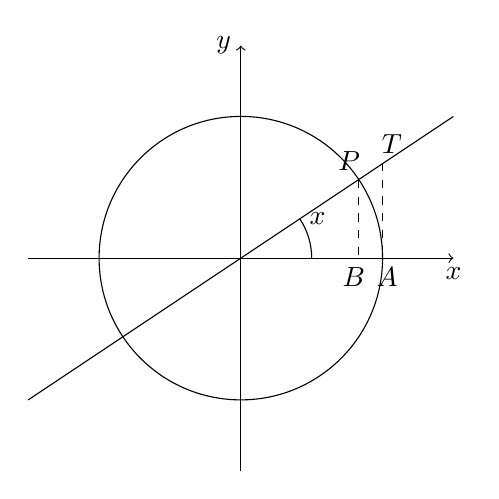
\begin{tikzpicture}[scale=1.8]
                \draw[->] (0,-1.5)--(0,1.5) node[left]{$y$};
                \draw[->] (-1.5,0)--(1.5,0) node[below]{$x$};
                \draw(0,0) circle (1);
                \draw(-1.5,-1)--(1.5,1);
                \draw(0.5,0) arc (0:33.7:0.5) node [right]{$x$};
                \draw[dashed](0.83,0.55) node [above] {$P~~$}to (0.83,0) node [below] {$B~$};
                \draw[dashed](1,0.67) node [above] {$~~T$}to (1,0) node [below] {$~A$};
            \end{tikzpicture}\\
        \caption{La situazione utilizzata per la dimostrazione}
        \label{fig:sinx}
    \end{figure}
    Per definizione si ha che \[\wideparen{PA}=x\]\[\overline{PB}=\sin x\] \[\overline{TA}=\tg x\] 
    Come è chiaramente visibile dalla Figura \ref{fig:sinx} si ha che \[\sin x < x < \tg x\] da cui \[\frac{\sin x}{\sin x}<\frac{ x}{\sin x}<\frac{\tg x}{\sin x}\] \[1<\frac{ x}{\sin x}<\frac{\tg x}{\sin x}\] \[1<\frac{\sin x}{x}<\cos x\]
    Si calcolano ora i limiti delle funzioni che limitano quella studiata
    \[\lim_{x \to 0^+}1=1 ~~~~~ \lim_{x \to 0^+}\cos x=1\]
    da cui per il teorema del confronto \[\lim_{x\to 0^+} \frac{\sin x}{x}=1\] Siccome la funzione è pari vale anche per $x\to0^-$
\end{proof}
\textbf{Osservazioni:}
\begin{itemize}
    \item vale il reciproco: $\lim_{x\to 0}\frac{x}{\sin x}=1$
    \item vale la generalizzazione: $\lim_{f(x)\to 0}\frac{\sin f(x)}{f(x)}=1$
    \item asintotico associato: $\sin x \sim x ~~~~\textnormal{in } I(0)$
\end{itemize}
\paragraph{$\lim_{x\to 0}\frac{\tg x}{x}=1$}~
\\\begin{proof}
    Per definizione $\tg x=\frac{\sin x}{\cos x}$, quindi \[\lim_{x\to 0} \frac{\tg x}{x}=\left[\frac{0}{0}\right]\overset{FI}{=}\lim_{x\to 0} \frac{\sin x}{x \cos x}\underset{LN}{=}\lim_{x\to 0} \frac{1}{\cos x}=1\]
\end{proof}
\textbf{Osservazioni:}
\begin{itemize}
    \item vale il reciproco: $\lim_{x\to 0}\frac{x}{\tg x}=1$
    \item vale la generalizzazione: $\lim_{f(x)\to 0}\frac{\tg f(x)}{f(x)}=1$
    \item asintotico associato: $\tg x \sim x ~~~~\textnormal{in } I(0)$
\end{itemize}

\subsubsection{$\lim_{x\to 0}\frac{1-\cos x}{x}=0$}
\begin{proof}
\[\lim_{x\to 0} \frac{1-\cos x}{x}=\left[\frac{0}{0}\right]\overset{FI}{=}\lim_{x\to 0}\frac{(1-\cos x)(1+\cos x)}{x(1+\cos x)}=\lim_{x\to 0}\frac{1-\cos^2 x}{x(1+\cos x)}=\]Per la prima relazione fondamentale della goniometria\[=\lim_{x\to 0}\frac{\sin^2 x}{x(1+\cos x)}\underset{LN}{=}\lim_{x\to 0}\frac{\sin x}{1+\cos x}=\left[\frac{0}{2}\right]=0\]
\end{proof}
\textbf{Osservazioni:}
\begin{itemize}
    \item NON vale il reciproco
    \item vale la generalizzazione: $\lim_{f(x)\to 0}\frac{1-\cos f(x)}{f(x)}=1$
\end{itemize}

\subsubsection{$\lim_{x\to 0}\frac{1-\cos x}{x^2}=\frac{1}{2}$}
\begin{proof}
\[\lim_{x\to 0} \frac{1-\cos x}{x^2}=\left[\frac{0}{0}\right]\overset{FI}{=}\lim_{x\to 0}\frac{(1-\cos x)(1+\cos x)}{x^2(1+\cos x)}=\lim_{x\to 0}\frac{1-\cos^2 x}{x^2(1+\cos x)}=\]Per la prima relazione fondamentale della goniometria\[=\lim_{x\to 0}\frac{\sin^2 x}{x^2(1+\cos x)}\underset{LN}{=}\lim_{x\to 0}\frac{1}{1+\cos x}=\frac{1}{2}\]
\end{proof}
\textbf{Osservazioni:}
\begin{itemize}
    \item vale il reciproco: $\lim_{x\to 0}\frac{x^2}{1-\cos x}=1$
    \item vale la generalizzazione: $\lim_{f(x)\to 0}\frac{1- \cos f(x)}{[f(x)]^2}=1$
    \item asintotico associato: $\cos x \sim 1 - x^2 ~~~~\textnormal{in } I(0)$
\end{itemize}

\subsubsection{$\lim_{x\to +\infty}\left(1+\frac{1}{x}\right)^{x} = e$}
\textbf{Osservazioni:}
\begin{itemize}
    \item NON vale il reciproco
    \item vale la generalizzazione
\end{itemize}

\paragraph{$\lim_{x\to +\infty}\left(1+\frac{k}{x}\right)^{x} = e^k$}~\\
\textbf{Osservazioni:}
\begin{itemize}
    \item NON vale il reciproco
    \item vale la generalizzazione
\end{itemize}

\paragraph{$\lim_{x\to 0^+}\left(1+kx\right)^{\frac{1}{x}}  e^k$}~\\
\textbf{Osservazioni:}
\begin{itemize}
    \item NON vale il reciproco
    \item vale la generalizzazione
\end{itemize}

\subsubsection{$\lim_{x\to 0}\frac{\log_a(1+x)}{x}=\log_ae=\frac{1}{\ln a}~~~~~~~~\textnormal{con }a>0$}
\begin{proof}
\[\lim_{x\to 0}\frac{\log_a(1+x)}{x}=\left[\frac{0}{0}\right]\overset{FI}{=}\lim_{x\to 0}\frac{1}{x}\log_a(1+x)=\lim_{x\to 0}\log_a(1+x)^\frac{1}{x}=\log_ae=\frac{\ln e}{\ln a}=\frac{1}{\ln a}\]
\end{proof}
Particolarizzazione: $\lim_{x\to0}\frac{\ln(1+x)}{x}=1$\\
\textbf{Osservazioni:}
\begin{itemize}
    \item vale il reciproco
    \item vale la generalizzazione
    \item asintotico associato: $\ln x \sim x - 1 ~~~~\textnormal{in } I(0)$
\end{itemize}

\subsubsection{$\lim_{x\to 0}\frac{a^x-1}{x}=\ln a~~~~~~~~\textnormal{con }a>0$}
\begin{proof}
Pongo $t=a^x-1$, quindi $e^x=t+1$ e di conseguenza $x=\log_a (t+1)$. Inoltre, se $x\to 0$, $t\to 0$.
\[\lim_{x\to 0}\frac{a^x-1}{x}=\lim_{t\to 0}\frac{t}{\log_a (t+1)}=\ln a\]
\end{proof}
Particolarizzazione: $\lim_{x\to 0}\frac{e^x-1}{x}=1$\\
\textbf{Osservazioni:}
\begin{itemize}
    \item vale il reciproco
    \item vale la generalizzazione
    \item asintotico associato: $e^x \sim x + 1 ~~~~\textnormal{in } I(0)$
\end{itemize}

\subsubsection{$\lim_{x\to 0}\frac{(1+x)^k-1}{x}=k$}
\textbf{Osservazioni:}
\begin{itemize}
    \item vale il reciproco
    \item vale la generalizzazione
    \item asintotico associato: $(1+x)^k \sim 1+kx ~~~~\textnormal{in } I(0)$
\end{itemize}
\section{Continuità e discontinuità}
\begin{tabular}{|m{0.3\textwidth}|m{0.6\textwidth}|}
        \hline
        Asintoto verticale&  \[\lim_{x\rightarrow x_0} f(x) = \infty\] \\\hline
        Asintoto orizzontale & \[\lim_{x\rightarrow \infty} f(x) = l\]\\ \hline
        Asintoto obliquo & \[\textnormal{CN: }\lim_{x\rightarrow\infty}f(x) = \infty\]
        \[m=\lim_{x\rightarrow\infty}\frac{f(x)}{x}\]
        \[q=\lim_{x\rightarrow\infty}f(x)-mx\] \\ \hline
    \end{tabular}\\
    \\
    \textbf{NB.:} Una funzione può avere anche infiniti asintoti verticali, ma al massimo due tra asintoti orizzontali e asintoti obliqui (uno destro e uno sinistro).\\    \begin{tabular}{|m{0.3\textwidth}|m{0.6\textwidth}|}
        \hline
        Prima specie &  \[\lim_{x\rightarrow x_0^-}f(x)=l_1~~~~\lim_{x\rightarrow x_0^+}f(x)=l_2\] \[l_1\neq l_2~~~~salto=|l_1-l_2|\]\\ \hline
        Seconda specie &  \[\lim_{x\rightarrow x_0^\pm}f(x)=\infty ~~~~\lor~~~~ \lim_{x\rightarrow x_0^\pm}f(x)=\nexists\] \\\hline
        Terza specie & \[\lim_{x\rightarrow x_0^-}f(x)=\lim_{x\rightarrow x_0^+}f(x)=l\]\[f(x_0)\neq l ~~~~ \lor ~~~~ f(x_0)=\nexists\]\\ \hline
    \end{tabular}
\subsection{Continuità e funzioni inverse}
    \subsubsection{Continuità della funzione inversa}
        \begin{shadedTheorem}[Continuità della funzione inversa]
            Se $y=f(x)$ è una funzione biiettiva e continua in un intervallo $D$, allora la funzione inversa $f^{-1}$ è continua nel codominio di $f$.
        \end{shadedTheorem}
        \begin{tabular}{m{0.45\textwidth}m{0.45\textwidth}}
            \textit{Ipotesi} & \textit{Tesi}  \\
            $f:D\to C$ biiettiva e continua in D & $f^{-1}:C\to D$ continua in C 
        \end{tabular}
        
    \subsubsection{Condizione di invertibilità per funzioni continue}
        \begin{shadedTheorem}[Invertibilità di funzioni continue]
            Sia $I$ un intervallo (limitato o illimitato) e $f:I\rightarrow \R$ una funzione continua in $I$. Allora essa è invertibile se e solo se è strettamente monotona.
        \end{shadedTheorem}
        \begin{tabular}{m{0.45\textwidth}m{0.45\textwidth}}
            \textit{Ipotesi} & \textit{Tesi}  \\
            $f:I\to \R$ continua e strettamente monotona in $I$ & $f$ è invertibile 
        \end{tabular}
    
\section{Teoremi sulle funzioni continue}
    \subsection{Teorema di Weistrass}
        \begin{shadedTheorem}[Weistrass]
            Se $f$ è una funzione continua in un intervallo limitato e chiuso $[a;b]$, allora essa assume in tale intervallo il massimo assoluto e il minimo assoluto.
        \end{shadedTheorem}
        \begin{tabular}{m{0.45\textwidth}m{0.45\textwidth}}
            \textit{Ipotesi} & \textit{Tesi}  \\
            $f:[a;b]\to \R$ continua in $[a;b]$ & $\exists c,d \in [a,b] : f(c) = min\{f\} \land f(d) = max\{f\}$
        \end{tabular}
    
    \subsection{Teorema dell'esistenza degli zeri (o di Bolzano)}
        \begin{shadedTheorem}[Bolzano]
            Se $f$ è continua in un intervallo limitato e chiuso $[a;b]$ e negli estremi di tale intervallo assume valori di segno opposto, allora esiste almeno un punto $c$ interno all'intervallo in cui $f(c)=0$.
        \end{shadedTheorem}
        \begin{tabular}{m{0.45\textwidth}m{0.45\textwidth}}
            \textit{Ipotesi} & \textit{Tesi}  \\
            \begin{enumerate}
                \item $f: [a;b] \to \R$ continua in $[a;b]$
                \item $f(a) \cdot f(b)<0$
            \end{enumerate} & $\exists c \in [a;b]:f(c)=0$ 
        \end{tabular}
    
    \subsection{Teorema dei valori intermedi (o di Darboux)}
        \begin{shadedTheorem}[Darbaux]
            Se $f$ è una funzione continua in un intervallo limitato e chiuso $[a;b]$, allora essa assume almeno una volta tutti i valori compresi tra il massimo e il minimo.
        \end{shadedTheorem}
        \begin{tabular}{m{0.45\textwidth}m{0.45\textwidth}}
            \textit{Ipotesi} & \textit{Tesi}  \\
            \begin{enumerate}
                \item $f: [a;b]\to \R$ continua in $[a;b]$
                \item $m=min\{[a;b]\}$ ~~~ $M=max\{[a;b]\}$
            \end{enumerate} & $\exists x \in [a,b] : f(x)=k \forall k \in [m;M]$
        \end{tabular}
\end{document}